\documentclass{article}

%titlepage

\title{my Titlepage}
\date{2013-09-01}
\author{Mario Koestl}


\usepackage{amsmath} % write contitions within the equations
\usepackage{graphicx} % for image insert, figure environment
\usepackage{placeins} % to use FloatBarrier
\usepackage{natbib} % to enable author name citations, and not only the reference
%
\usepackage{booktabs} % to make tables prettier
\usepackage{listings} % for code insertion
\usepackage{color} % for syntax highlighting



\begin{document}
\pagenumbering{gobble} % no numberin on the titlepage
\maketitle
\newpage
\pagenumbering{arabic} % or roman

%\chapter{overall view} can be used with report
\section{equations}

%formulas with equation section or..
\begin{equation}
f(x) = 
\begin{cases}
\frac{1}{x^2} * \sqrt[8]{3},& \text{if } x\geq 1\\
1, & \text{if } x < 1\\
\end{cases}
\end{equation}

%or with the $$ area
$\sum^n_{i=1}$

% alignmentsvon formeln gehen auch so
\begin{align*}
  g(x) &= \frac{1}{x}\\
  F(x) &= \int^a_b \frac{1}{3}x^3
\end{align*}


\subsection{figures}
Now insert some figures into the document

I creates 2 pictures and the refrence to this pictures = \ref{fig:2pictures}

%[h] defines where the figure should be on the page
%h (here) - same location
%t (top) - top of page
%b (bottom) - bottom of page
%p (page) - on an extra page
%! (override) - will force the specified location

\begin{figure}[b] 
 
  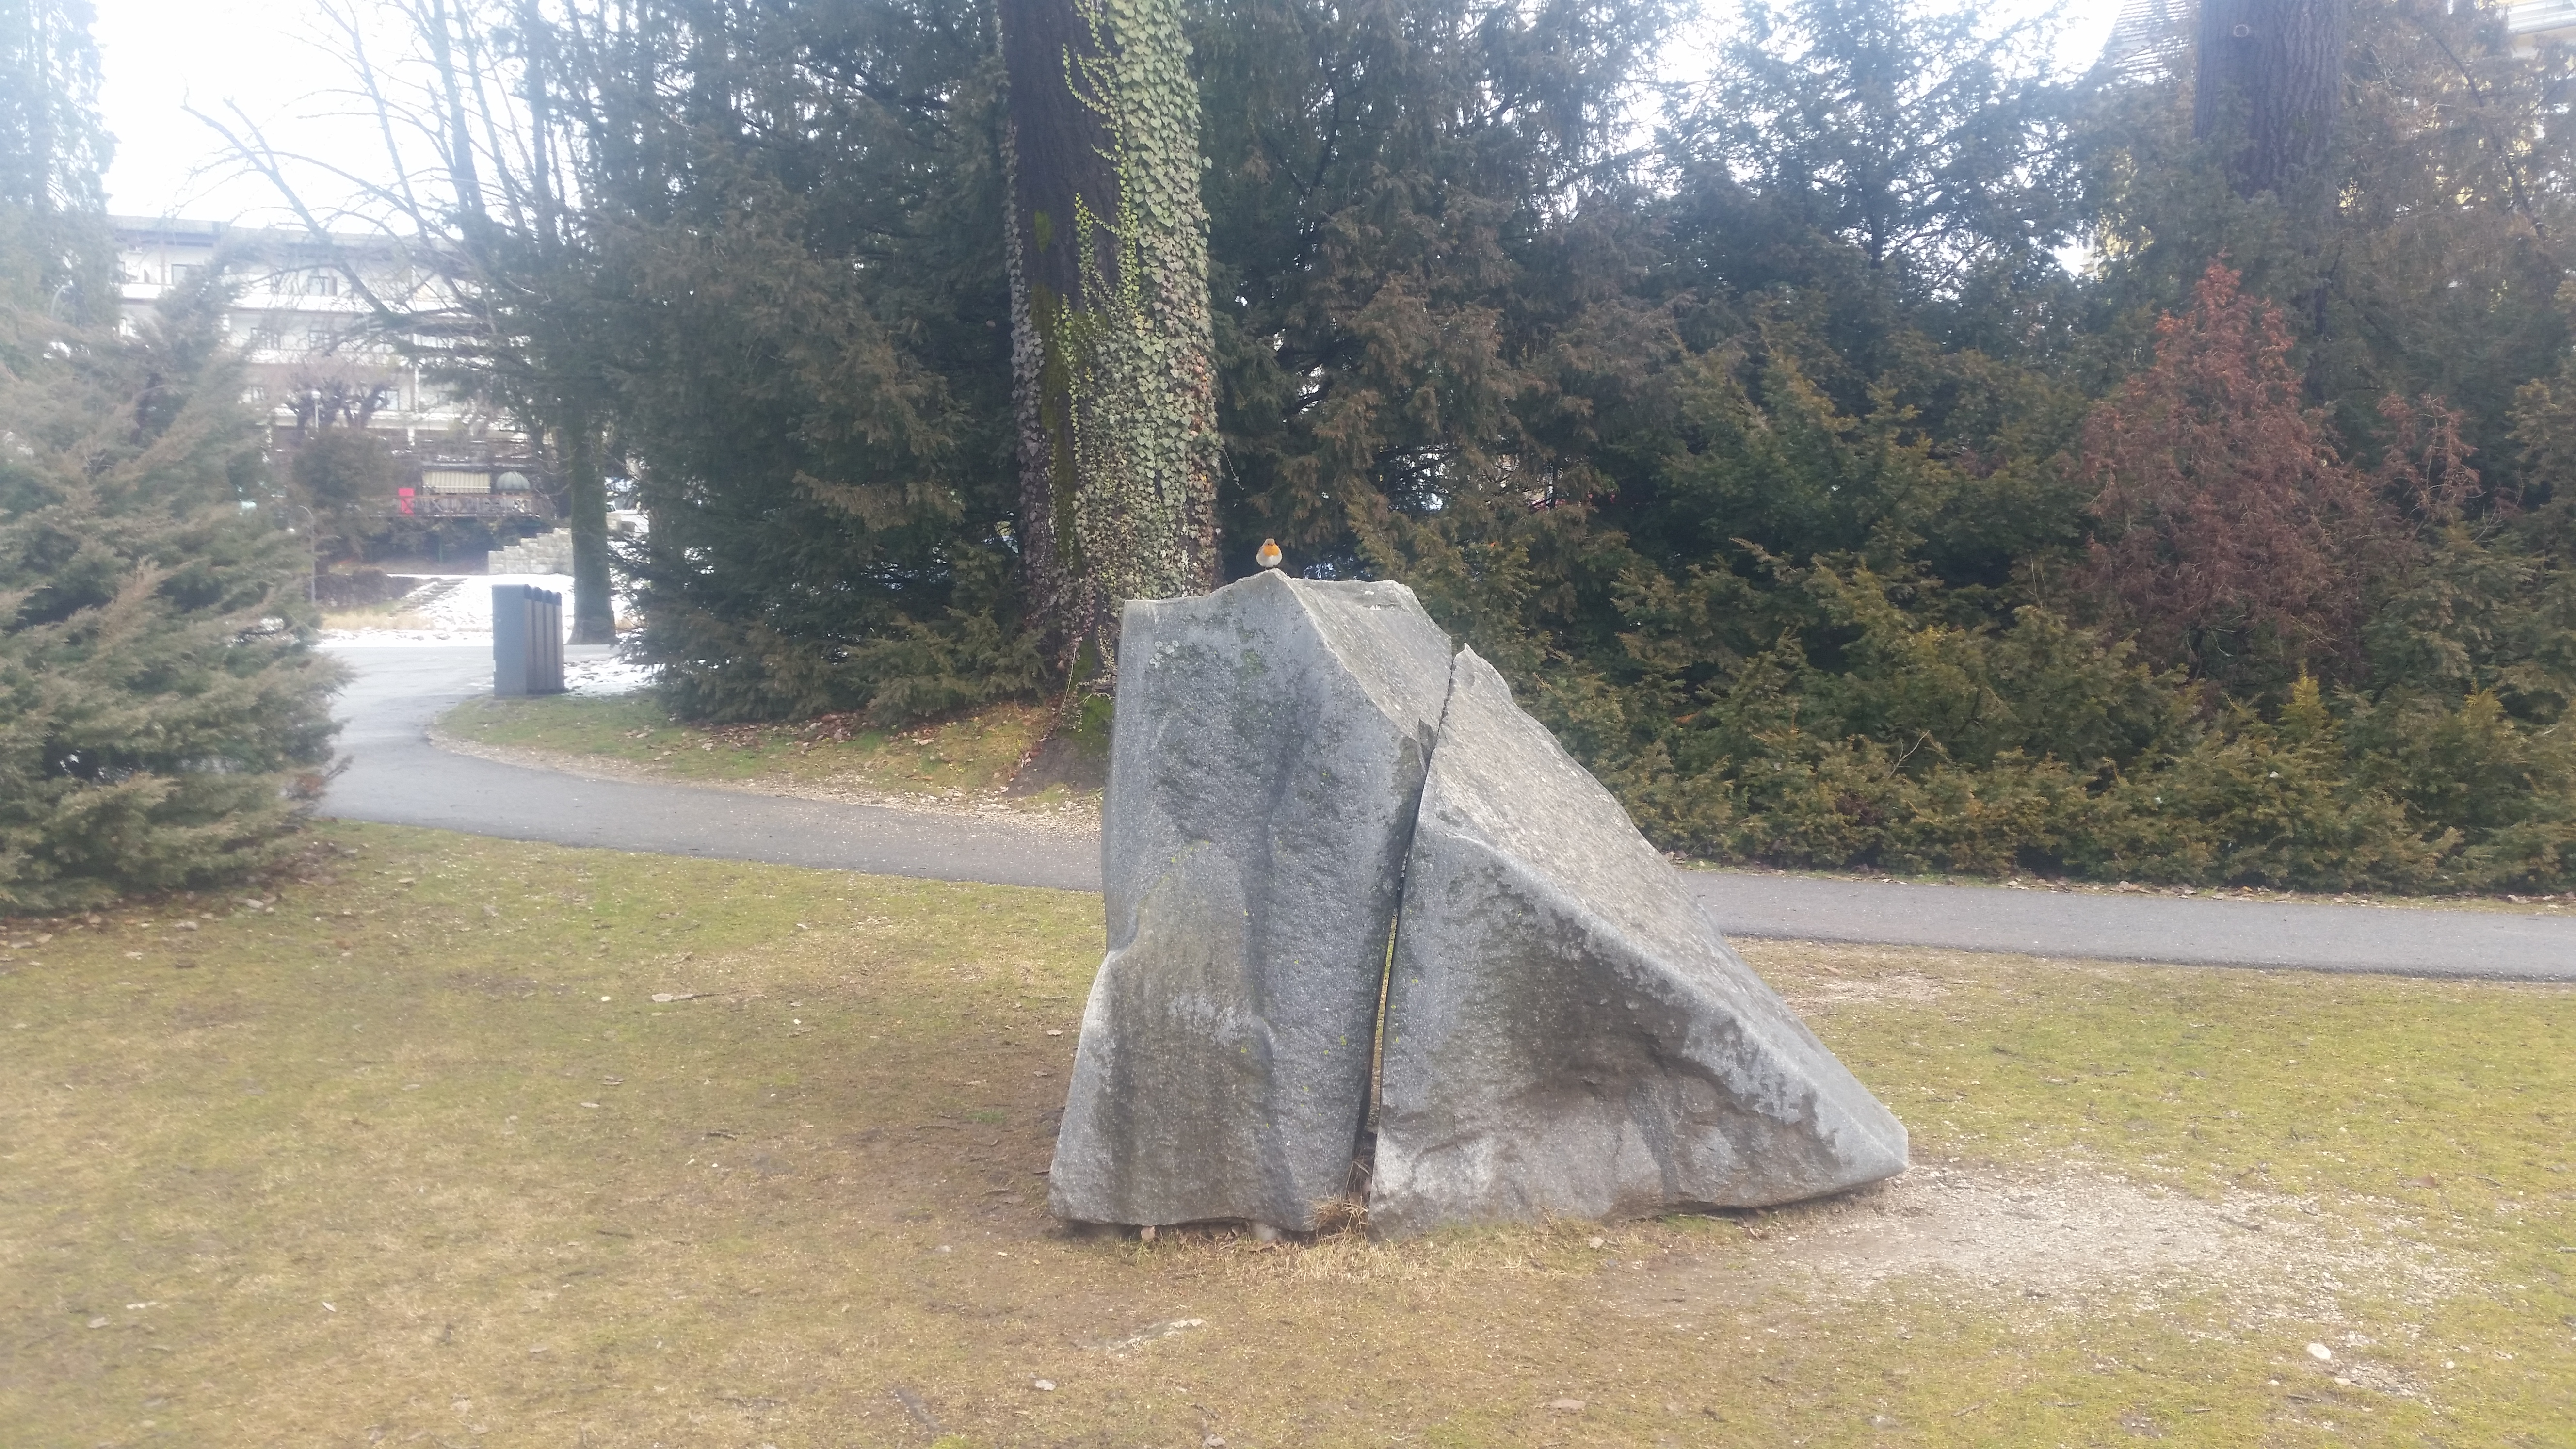
\includegraphics[width=0.3\linewidth, angle = 180]{test.jpg}
  %%or with cm 
  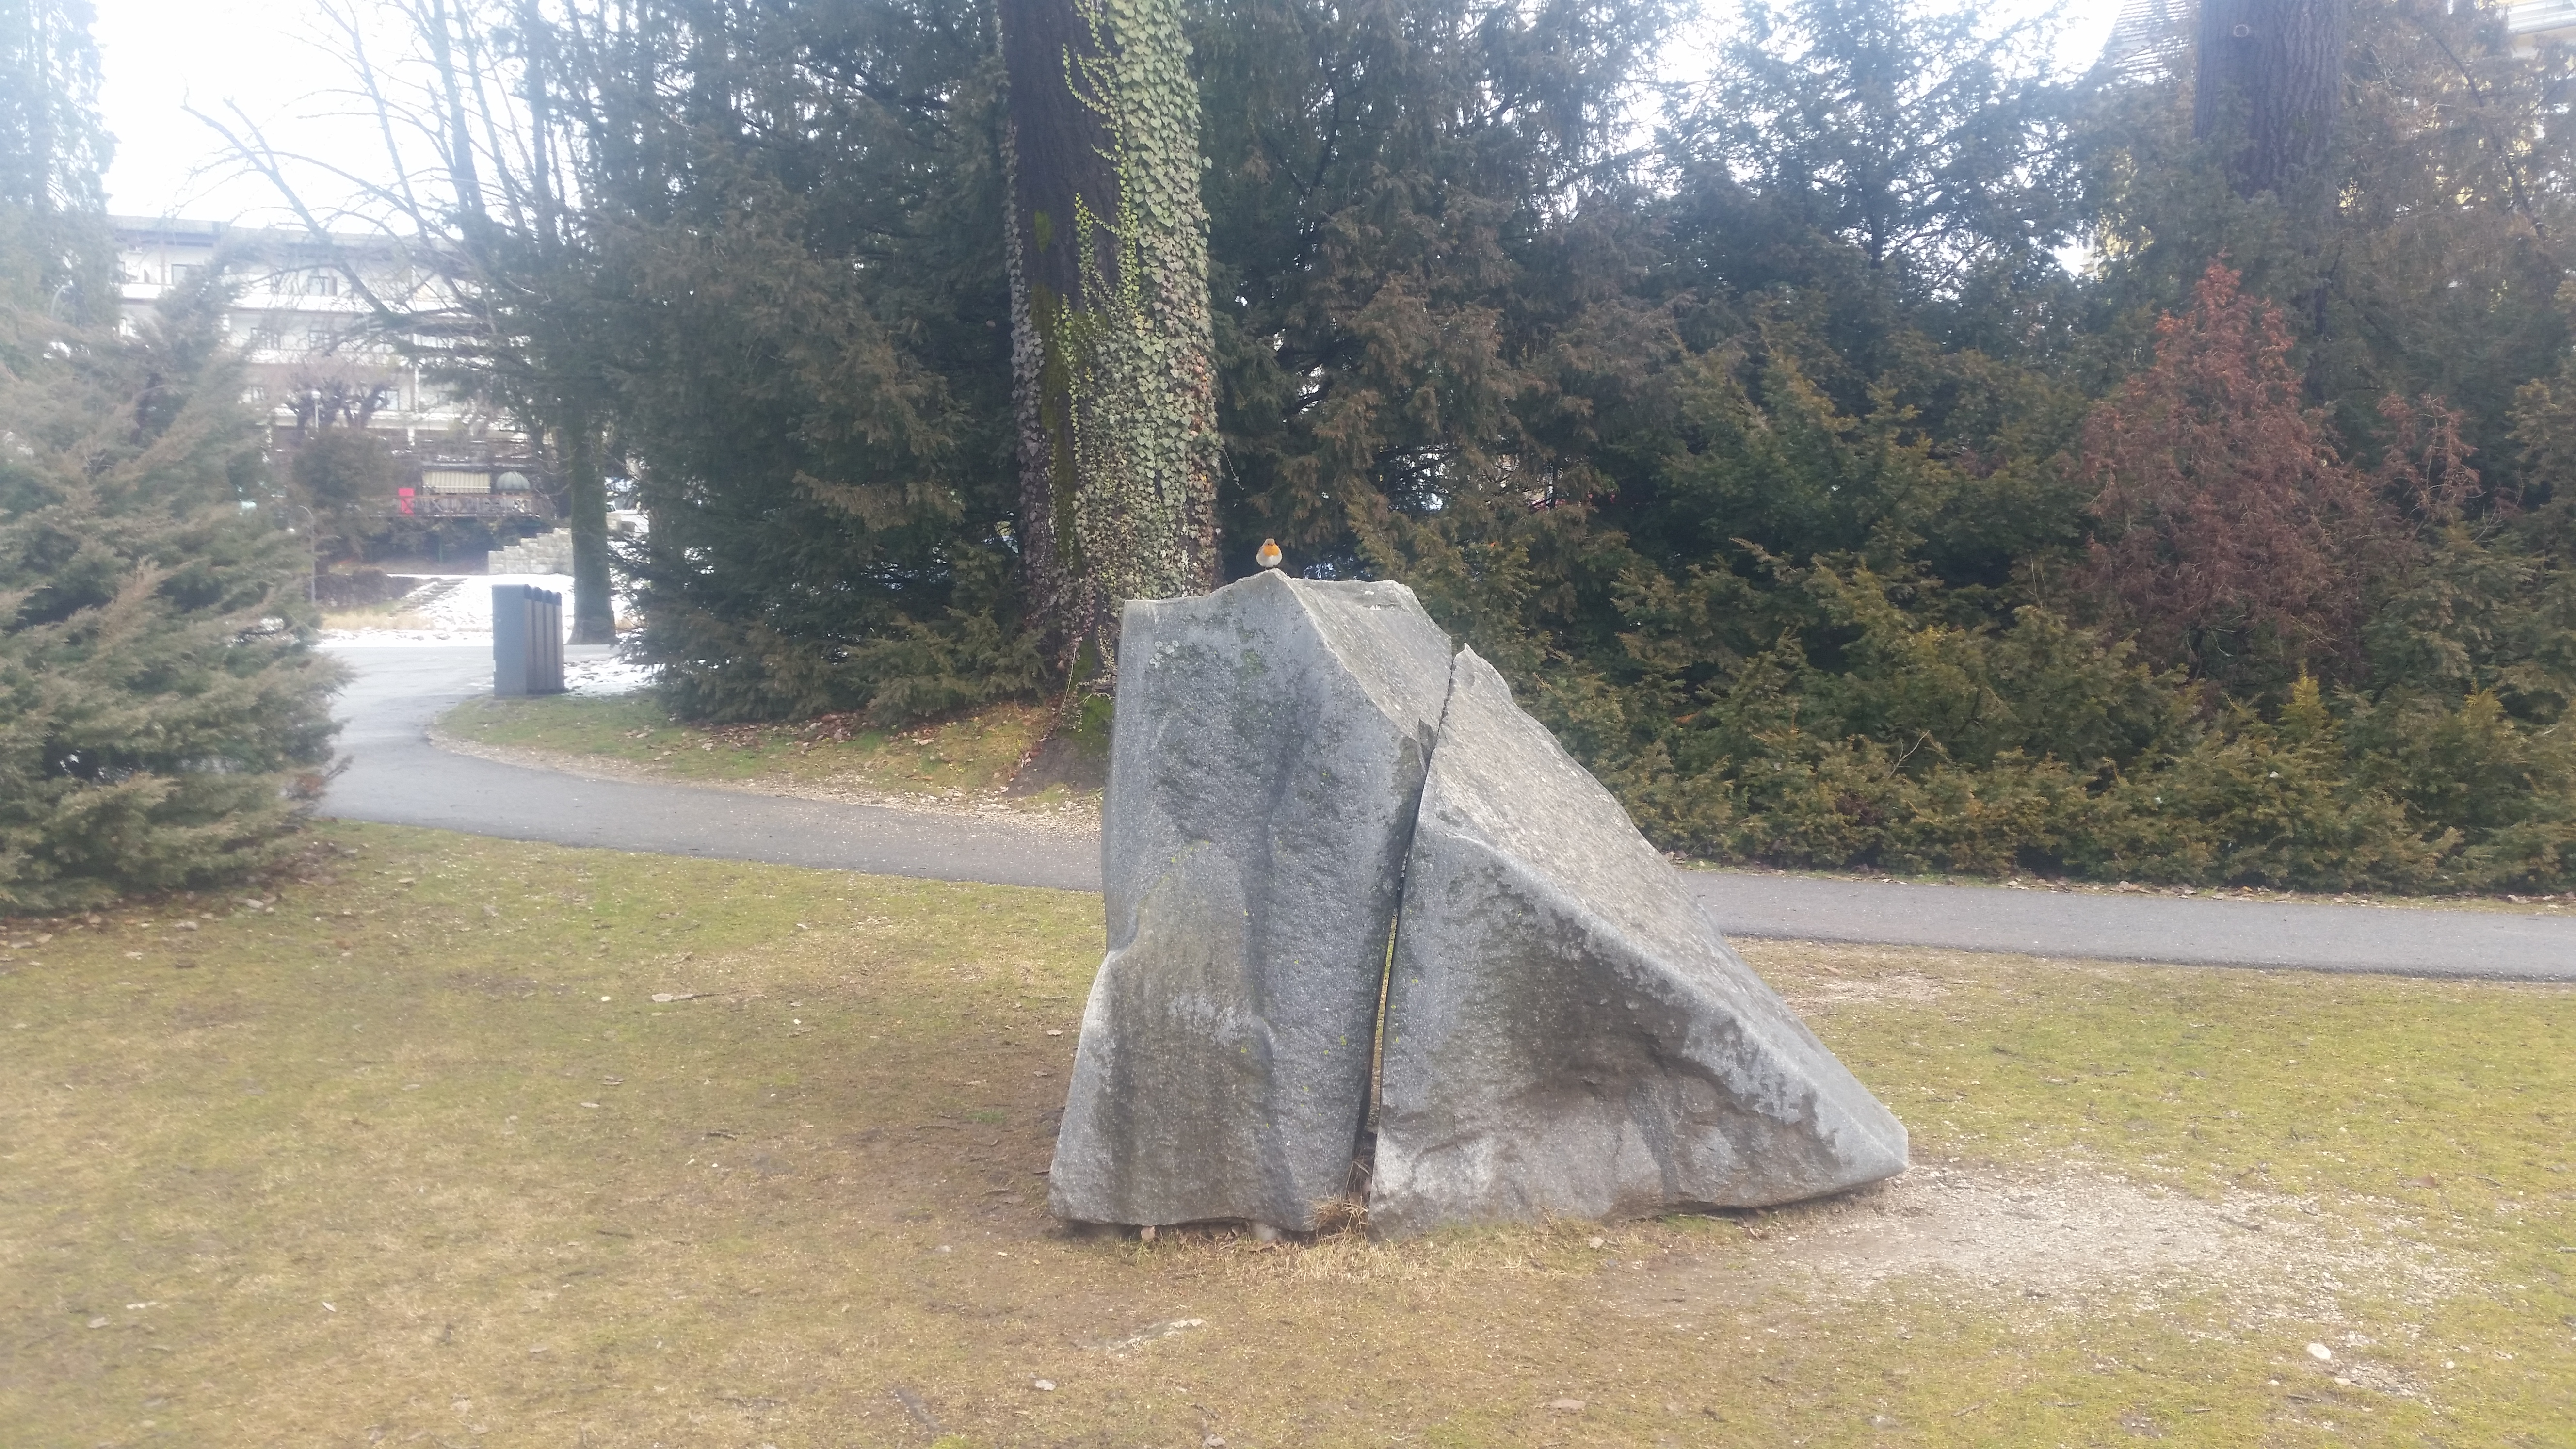
\includegraphics[width=5.25cm,height=5.25cm]{test.jpg}
  \caption{2 pictures.}
  \label{fig:2pictures}
\end{figure}

\FloatBarrier % automatically arranged float pictures cannot go over this line
\subsubsection{citation usage}
OFTEN IT IS NECCESSARY TO DELETE THE AUX AND BBL FILE
Random citation  \citet{DUMMY:1} embeddeed in text.
multiple citations \cite{DUMMY:2,DUMMY:1}.
%Citation with name of author, from natbib \cite{DUMMY:1}.

\paragraph{para 1}
\subparagraph{subpara1}
 
\subsubsection{autofootnotes} 
%https://www.latex-tutorial.com/tutorials/beginners/latex-bibtex/
i cannot use this simultanious with natbib, why not
%\usepackage[backend=bibtex,style=verbose-trad2]{biblatex}
%\bibliography{marioBib} % define the used bib file
%Random citation \autocite[1]{DUMMY:1} embeddeed in text.


\subsubsection{references to footnotes}
\footnote{\label{myfootnote}Hello footnote}

Tihs is a reference to the footnote \ref{myfootnote}.

calcultions show a drop in Figure:\ref{fig:2pictures}, and is therefore bad.
\tableofcontents % 
\newpage


\section{Tables}

\begin{table}[h!]
  \centering
  \caption{Caption for the table.}
  \label{tab:table1}
  \begin{tabular}{l|c||r} % left|center|right, could be other things, can even be cm
    1 & 2 & 3\\
    \hline
    a & b & c\\
  \end{tabular}
\end{table}

with booktabs

\begin{table}[h!]
  \centering
  \caption{Caption for the table.}
  \label{tab:table1:extended}
  \begin{tabular}{l|c||r} % left|center|right, could be other things, can even be cm
  \toprule
  	\multicolumn{3}{c}{Title things} \\ % multicolumns to merge columns
  \midrule
    1 & 2 & 3\\
    \hline
    a & b & c\\
  \bottomrule  
  \end{tabular}
\end{table}


get a table from a csv file :

https://www.latex-tutorial.com/tutorials/advanced/latex-pgfplotstable/


\section{code insertions}

%\usepackage{listings} % for code insertion
%\usepackage{color} % for syntax highlighting
\lstset{ % General setup for the package
	language=Perl,
	basicstyle=\small\sffamily,
	numbers=left,
 	numberstyle=\tiny,
	frame=tb,
	tabsize=4,
	columns=fixed,
	showstringspaces=false,
	showtabs=false,
	keepspaces,
	commentstyle=\color{red},
	keywordstyle=\color{blue}
}

\begin{lstlisting}
#!/usr/bin/perl
print S(@ARGV);
sub S{
	$r=@_[0];
return $r;
}
\end{lstlisting}

%or yust use an existing file if available 
%\lstinputlisting{script.pl}


%appendix
 \begin{appendix}
  \listoffigures
  \listoftables
 \end{appendix}

%bibliography things
\bibliography{marioBib} % define the used bib file
\bibliographystyle{plainnat} %define a style
%ieeetr, without natbib
%plainnat 






\end{document}